\documentclass[a4paper]{article}
\usepackage[procnames]{listings}
\usepackage{color}
\usepackage{graphicx}
\begin{document}
\definecolor{keywords}{RGB}{255,0,90}
\definecolor{comments}{RGB}{0,0,113}
\definecolor{red}{RGB}{160,0,0}
\definecolor{green}{RGB}{0,150,0}
\graphicspath{ {/Users/wangbochen/GitHub/ModernAnalysis/HW1/Digit/} }
\lstset{language=Python, 
        basicstyle=\ttfamily\small, 
        keywordstyle=\color{keywords},
        commentstyle=\color{comments},
        stringstyle=\color{red},
        showstringspaces=false,
        identifierstyle=\color{green},
        procnamekeys={def,class}}

\title{Digits}
\author{Tianyuan Liu, Bochen Wang}
\maketitle
\section*{Introduction}
This is the first part of programming assignment 1.
\section*{Implementation}
\subsection*{Import Libraries}
Import the necessary libraries we need.
\begin{lstlisting}
import numpy as np
import pylab
from MyKNearestNeighborClassifier import MyKNNClassifier as KNeighborsClassifier
from sklearn import cross_validation
import sys  
\end{lstlisting}
\subsection*{Data Reading}
Load the train data and train label into memory.
\begin{lstlisting}
#Part a
#Read train data and train label.
raw_tr_data = np.loadtxt(open("train.csv","rb"),delimiter=",",skiprows=1)
train_label = raw_tr_data[:,0]
train_data = raw_tr_data[:,1:]
neighbos_num = 9
\end{lstlisting}
\subsection*{Digit Display}
Display one of each digit.
\begin{lstlisting}
#Part b
#The function display_digit is implemented to display a digit.
def display_digit(label,X,colormap=pylab.cm.gist_gray):
    l = len(X)
    m = int(np.ceil(np.sqrt(l)))
    M = np.zeros((m,m)) 
    for i in range(m):
        M[i,:] = X[i*m:(i+1)*m]
    pylab.imshow(M, cmap=colormap)
    pylab.imsave(str(label)+".png",M)    
    pylab.axis('off')
    return M

#Display one digit of each class.
record = {}
index = 0
for i in range(len(train_label)):
    if len(record) == 10:
        break
    if not record.has_key(index):
        display_digit(train_label[index],train_data[index])
        record[train_label[index]] = index
    index = index + 1
\end{lstlisting}

\subsection*{Digits Count Distribution}
Plot a histogram of digits count in training data set.
\begin{lstlisting}
#Part c
#Plot a histogram of digits count in training data set.
digit_count = np.zeros((10))
for i in range(len(train_label)):
    index = int(train_label[i])
    digit_count[index] = digit_count[index] + 1

pr_distribute = digit_count/len(train_label)
pylab.hist(train_label,align="mid",rwidth=0.8);
\end{lstlisting}
\begin{center}
The Distribution of the Digits Count
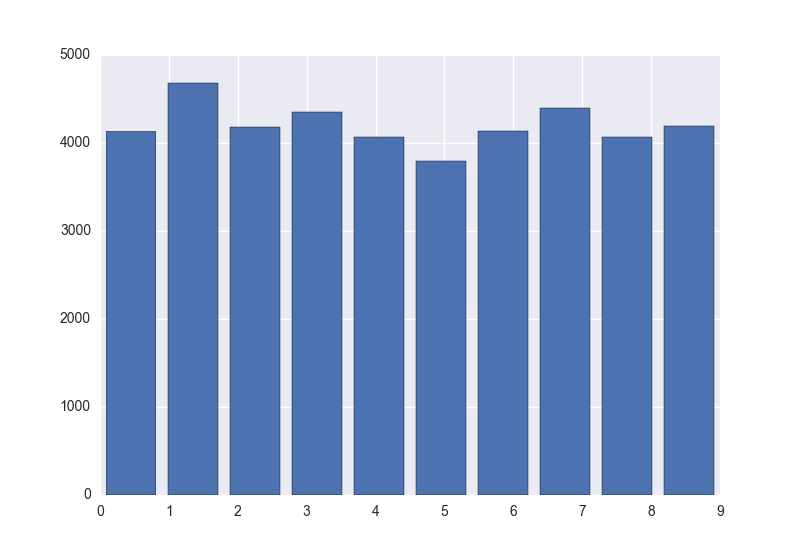
\includegraphics[scale=0.63]{digit_histogram.png}
\end{center}

\subsection*{Find Nearest Neighbor}
Find the nearest neighbor of each digit.
\begin{lstlisting}
#Part d
#Find the nearest neighbor of sample digits in train data set.
#The result shows that there is no erroneous example.
ret = np.zeros((10))
for i in range(10):
    index = record[i]
    maxdist = sys.maxint
    for j in range(len(train_label)):
        if j == index:
            continue
        dist = np.linalg.norm(train_data[j][:]-train_data[index][:])
        if dist < maxdist:
            maxdist = dist
            ret[i] = j
            
for i in range(10):
    print(train_label[ret[i]])
\end{lstlisting}
The result is:
\begin{center}
\begin{tabular}{llllllllll}
\hline
	0.0 & 1.0 & 2.0 & 3.0 & 4.0 & 5.0 & 6.0 & 7.0 & 8.0 & 9.0 \\
\hline
\end{tabular}
\end{center}

\subsection*{Pairwise Distances Distribution}
Compute all the genuine pairwise distances and imposter pairwise distances.
\begin{lstlisting}
#Part e
#Compute all the genuine pairwise distances and imposter pairwise distances.
train_zero = []
train_one = []
for i in range(len(train_label)):
    if train_label[i] == 0:
        train_zero.append(train_data[i][:])
    if train_label[i] == 1:
        train_one.append(train_data[i][:]) 
train_zero_one = [train_zero,train_one]
genuine_pairwise_distance = []
imposter_pairwise_distance = []
for k in range(2):
    length = np.shape((train_zero_one[k]))[0]
    for i in range(length):
        for j in range(i+1,length):
            temp = np.linalg.norm(train_zero_one[k][i]-train_zero_one[k][j])
            genuine_pairwise_distance.append(temp)
length_zero = np.shape(train_zero)[0]
length_one = np.shape(train_one)[0]
for i in range(length_one):
    for j in range(length_zero):
        temp = np.linalg.norm(train_one[i]-train_zero[j])
        imposter_pairwise_distance.append(temp)
\end{lstlisting}
Plot a histogram to show the distribution of both kinds of pairwise of distances.
\begin{lstlisting}
#Plot a histogram to show the distribution of both kinds of pairwise distances.
pylab.hist((genuine_pairwise_distance,imposter_pairwise_distance), 500, 
	normed=True, histtype="step")
\end{lstlisting}
\begin{center}
The Distribution of the Pairwise Distances
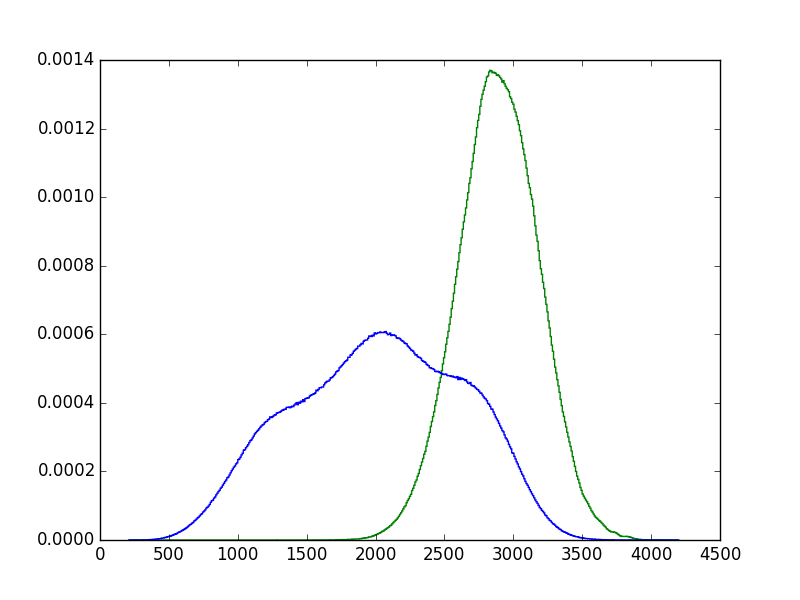
\includegraphics[scale=0.63]{pairwise_distance.png}
\end{center}

\subsection*{ROC Curve and Equal Error Rate}
Plot the ROC curve according to the pairwise distances.
\begin{lstlisting}
#Part f
#Plot the ROC curve according to the pairwise distances.
genuine_pairwise_distance.sort()
imposter_pairwise_distance.sort()
def b_search(x,arr):
    i = 0
    j = len(arr)-1
    closest = arr[j]
    closest_index = 0
    while i < j:
        mid = (i + j)/2
        temp = abs(arr[mid]-x)
        if temp < closest:
            closest = temp
            closest_index = mid
        if arr[mid] >= x:
            j = mid - 1
        if arr[mid] < x:
            i = mid + 1
    return closest_index  
def calculate_rate(threshold,genuine,impost):
    fp_count = len(genuine) - b_search(threshold,genuine_pairwise_distance)
    tp_count = len(impost) - b_search(threshold,imposter_pairwise_distance)
    fp_rate = float(fp_count)/len(genuine)
    tp_rate = float(tp_count)/len(impost)
    return fp_rate,tp_rate
false_positive_rate = []
true_positive_rate = []
ts = []
threshold = 0
upper_limit = int(min(genuine_pairwise_distance[-1],imposter_pairwise_distance[-1]))
step = upper_limit/500
while threshold < upper_limit:
    ts.append(threshold)
    fp,tp = calculate_rate(threshold,genuine_pairwise_distance,imposter_pairwise_distance)
    false_positive_rate.append(fp)
    true_positive_rate.append(tp)
    threshold += step
roc_fig = pylab.figure()
pylab.plot(false_positive_rate,true_positive_rate)
pylab.xlabel("False Positive Rate")
pylab.ylabel("True Positive Rate")
pylab.show()
\end{lstlisting}
\begin{center}
ROC Curve of Pairwise Distances
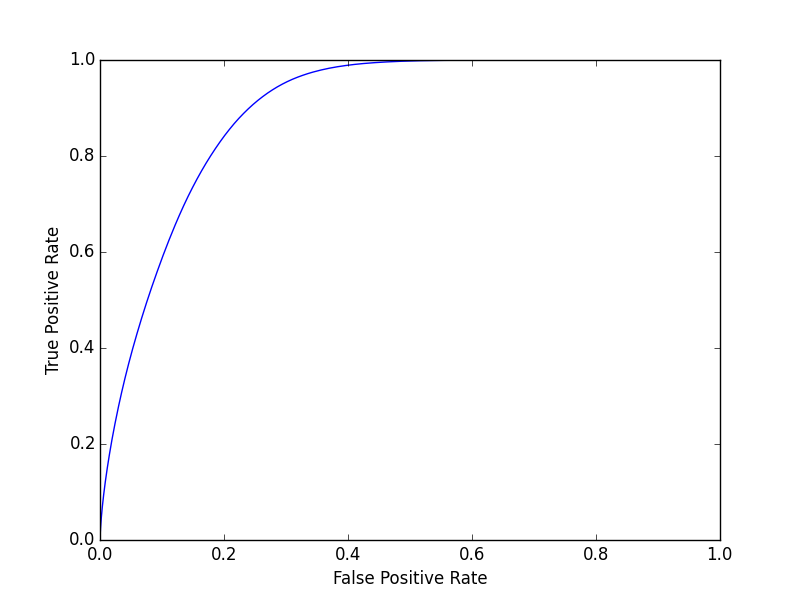
\includegraphics[scale=0.63]{ROC_Curve.png}
\end{center}
Find the equal error rate of the pairwise distances.
\begin{lstlisting}
#Find the equal error rate of the pairwise distances.
false_match_rate = false_positive_rate
false_none_match_rate = []
for e in true_positive_rate:
    false_none_match_rate.append(1-e)
pylab.plot(ts,false_match_rate)
pylab.plot(ts,false_none_match_rate)
#The Equal Error Rate is around 2640
#The Equal Errot Rate of random classifier is around 2250
\end{lstlisting}
\begin{center}
FMR(False Match Rate) vs FNMR(False None Match Rate)
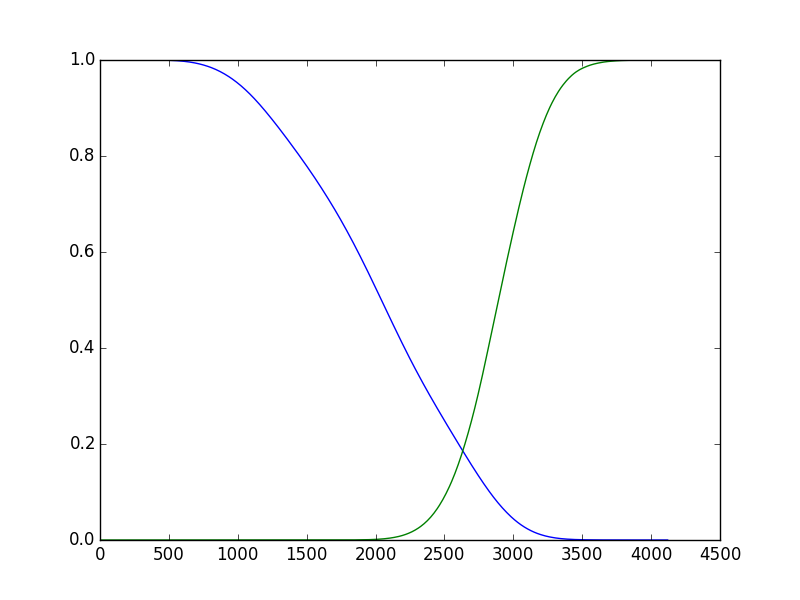
\includegraphics[scale=0.63]{Equal_Error_Rate.png}
\end{center}

\subsection*{Implement KNN Classifier}
Use KDTree in scipy to implement the KNN classifier.
\begin{lstlisting}
#Part g
#Implement KNN Classifier
import numpy as np
from scipy import spatial as spt
class MyKNNClassifier(object):
    def __init__(self,k):
        self.k = k        
    def fit(self,train_data,train_label):
        self.kdTree = spt.KDTree(train_data)
        self.label = train_label        
    def predict(self,test_data):
        res = self.kdTree.query(test_data,self.k)
        test_label = self.label[res[1]]
        ret = []
        for e in test_label:           
            count_map = {}
            print(e)
            for label in e:
                if count_map.has_key(label):
                    count_map[label] += 1;
                else:
                    count_map[label] = 1;            
            max_val = 0
            max_label = 0
            for e in count_map:
                if count_map[e] > max_val:
                    max_val = count_map[e]
                    max_label = e
            ret.append(max_label)      
        return np.array(ret)
\end{lstlisting}
\subsection*{Cross Validation and Confusion Matrix}
Implement 3-fold cross validation on training data set and generate the confusion matrix.

\begin{lstlisting}
#Part h and i
#Implement 3-fold cross validation on train data set.
#Generate the confusion matrix
folds_num = 3
confusion = np.zeros((10,10)) 
kf = cross_validation.KFold(len(train_label), n_folds=folds_num)
pr_sum = 0;
for train_index, test_index in kf:
    train_data_fold, test_data_fold = train_data[train_index], 
    	train_data[test_index]
    train_label_fold, test_label_fold = train_label[train_index], 
    	train_label[test_index]
    neigh = KNeighborsClassifier(neighbos_num)
    neigh.fit(train_data_fold,train_label_fold)
    res = neigh.predict(test_data_fold)
    for i in range(0,len(res)):
        confusion[test_label_fold[i]][res[i]] += 1
    correct_vec = res-test_label_fold
    correct_count = 0
    for e in correct_vec:
        if e == 0:
            correct_count += 1
    pr = float(correct_count)/len(test_label_fold)
    pr_sum += pr
    print(pr)

avg_correct = pr_sum/folds_num
print(avg_correct)
print(confusion)
mis_classified = []
for i in range(10):
    temp = 0;
    for j in range(10):
        if i != j:
            temp += confusion[i][j]
    mis_classified.append(temp)
print(mis_classified)
#KNN classifier 3-fold cross validation average accuracy = 0.9631
#tricky rank
# 8 2 4 9 3 5 7 6 1 0
\end{lstlisting}

\subsection*{Prediction}
Train the classifier with whole training data set and predict the test data.
\begin{lstlisting}
#Part j
#Train the classifier with whole train data set and predict the test data.
test_data = np.loadtxt(open("test.csv","rb"),delimiter=",",skiprows=1)
neigh = KNeighborsClassifier(neighbos_num)
neigh.fit(train_data,train_label)
predict_res = neigh.predict(test_data)
predict_res = predict_res.astype(int)
image_id = np.array(range(1,len(predict_res)+1))
save_arr = np.vstack((image_id,predict_res))
np.savetxt("test_res.csv", np.transpose(save_arr), delimiter=",",fmt="%d")
\end{lstlisting}
This is our final Kaggle rank:
\begin{center}
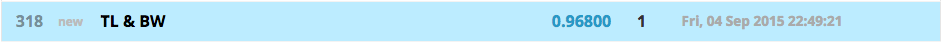
\includegraphics[scale=0.45]{Kaggle_Rank.png}
\end{center}





















\end{document}